\documentclass[rmp,twocolumn]{revtex4}
\usepackage[english]{babel}
\usepackage{amssymb,amsfonts,amsmath}
\usepackage{color}
\usepackage{graphicx}
\usepackage{amsmath}
\usepackage{natbib}
\usepackage{hyperref}
\usepackage{enumerate}

% Code syntax highlighting
\usepackage{listings}
\lstloadlanguages{C++,Python}

\newcommand{\EQ}[1]{Eq.~(\ref{eq:#1})}
\newcommand{\EQS}[2]{Eqs.~(\ref{eq:#1}) and (\ref{eq:#2})}
\newcommand{\FIG}[1]{Fig.~\ref{fig:#1}}
\newcommand{\TAB}[1]{Tab.~\ref{tab:#1}}
\newcommand{\REF}[1]{ref.~\citep{#1}}

\newcommand{\comment}[1]{{\color{red}#1}}

\newcommand{\mut}{u}
\newcommand{\mfit}{\langle F\rangle}
\newcommand{\mexpfit}{\langle e^{F}\rangle}
\newcommand{\ox}{r}
\newcommand{\co}{\rho}
\newcommand{\gt}{g}
\newcommand{\fcoeff}{f}
\newcommand{\locus}{s}
\newcommand{\locuspm}{t}
\newcommand{\OO}{\mathcal{O}}

\definecolor{dkgreen}{rgb}{0,0.6,0}
\definecolor{gray}{rgb}{0.5,0.5,0.5}
\definecolor{mauve}{rgb}{0.58,0,0.42}

%%%%%%%%%%%%%%%%%%%%%%%%%%%%%%%%%%%%%%%%%%%%%%%%%%%%%%%%%%%%%%%%%%%%%%%%%%%%%%
\begin{document}
%%%%%%%%%%%%%%%%%%%%%%%%%%%%%%%%%%%%%%%%%%%%%%%%%%%%%%%%%%%%%%%%%%%%%%%%%%%%%%
\title{Inferring selection coefficients from multi-locus genotype data:
Applications to HIV}
%\author{Taylor~Kessinger}
%\author{Richard~A.~Neher}
%\affiliation{Max Planck Institute for Developmental Biology, 72076 T\"ubingen,
% Germany}
%\affiliation{${}^{\dagger}$ Fachbereich Bioinformatik, University of
%T\"ubingen, Germany}


\date{\today}

%%%%%%%%%%%%%%%%%%%%%%%%%%%%%%%%%%%%%%%%%%%%%%%%%%%%%%%%%%%%%%%%%%%%%%%%%%%%%%
\begin{abstract}

\end{abstract}
\maketitle
During the first couple of month of an HIV infection, the viral genome typically
undergoes a series of rapid amino acid substitutions that reduce immune
pressure by cytotoxic T-lymphocytes (CTL), so called CTL escape
\citep{Mcmichael:2009p31614}. The substitutions arise by random mutation and
spread through the population since they impair the presentation of the epitope
in on the cell surface or the recognition of the MHC-epitope complex by T-cell
receptors. Avoiding recognition is an obvious benefit to the mutant virus, but
escape mutations can interfere with process necessary for virus replication and
infection and thereby reduce the intrinsic fitness REF. The rate at which escape
variants displace the founder sequences depends on both the ``avoided killing''
and the fitness cost. To quantify the role of individual CTL clones in
controlling the viral population and the fitness costs associated with escape
mutations, one would often like to infer the growth rate associated
with the individual mutations from serially sampled sequence data.

With a single escape mutation and dense and deeply sampled data, the escape rate
can simply be estimated by fitting a logistic curve to the time course of the
frequency of the mutation \citep{Asquith:2006p28003,Ganusov:2011p43139}. The
logistic curve has two parameters, the growth or escape rate, and the frequency
at the initial time point. In many cases, however, the data obtained from
infected patients is scarce and estimating two parameters reliably from the data
is not possible \citep{Ganusov:2011p43139}. \FIG{data_example} shows an example
of such time series sequence data of CTL escape of HIV. The data is rather
sparse and the sampling depth is low. Furthermore, not only one single escape mutation is observed, but
several mutations rapidly emerge in different places in the viral genome
\citep{Goonetilleke:2009p42296,SalazarGonzalez:2009p35091}. Multiple escapes
imply immune pressure on many epitopes. Since the viral population and its
mutation rate are large \citep{Perelson:1996p23158,Mansky:1995p38971}, these
different escape mutations will arise simultaneously. Initially, these escape
mutations exist in the population as single mutant genomes until they are
combined into mutliple mutants by recurrent mutation or recombination
\citep{ganusov_mathematical_2013}. This competition affects the trajectories of
individual escape mutations and estimating their intrinsic growth rate by
logistic fitting is not accurate. The degree of competition between genotypes
depends on the population size, the mutation rate, and the recombination rate in
HIV populations. The latter is rather low
\citep{Neher:2010p32691,Batorsky:2011p40107}, and it has been shown that
strong selection such as drug resistance selection changes affects mutations
along the entire genome \citep{Nijhuis:1998p44376}.

Here, we develop a inference strategy that allows to obtain robust estimates
from scarce data typical of studies of CTL escape. The inference is based on
explicit modeling of the process of accumulation of mutations on the founder
sequence. Thereby, we exploit contraints imposed by the underlying dynamics of
mutation and selection in the high dimensional space of possible genotypes. As a
result, the estimates are much more robust. 

Despite the large number of possible genomes that can be formed from different
combination of escape mutations, we typically observe one or two dominant
genotypes. Furthermore, these genotypes dominate only transiently and are
quickly displaced by genotypes with an even greater number of escape mutations;
see \FIG{data_example}. Given a data set, it is typically straightforward to
define a series of dominant genotypes that likely have arisen by through
step-wise accumulation of mutations -- either through do novo mutation or
recombination. In many cases, the first few CTL escapes are very rapid and the
viral population is large, such that recombination only plays a minor role in
the accumulation. In \ref{Ganusov:2012}, a frame work for multi-locus modeling
of CTL escape is presented. Building on this framework, we explicitly model the
transition from one dominant genotype to another. The restriction to dominant
genotypes captures the interference between different loci, while avoiding
the need to solve the full multi-locus problem.


%\usepackage{graphics} is needed for \includegraphics
\begin{figure}[htp]
\begin{center}
  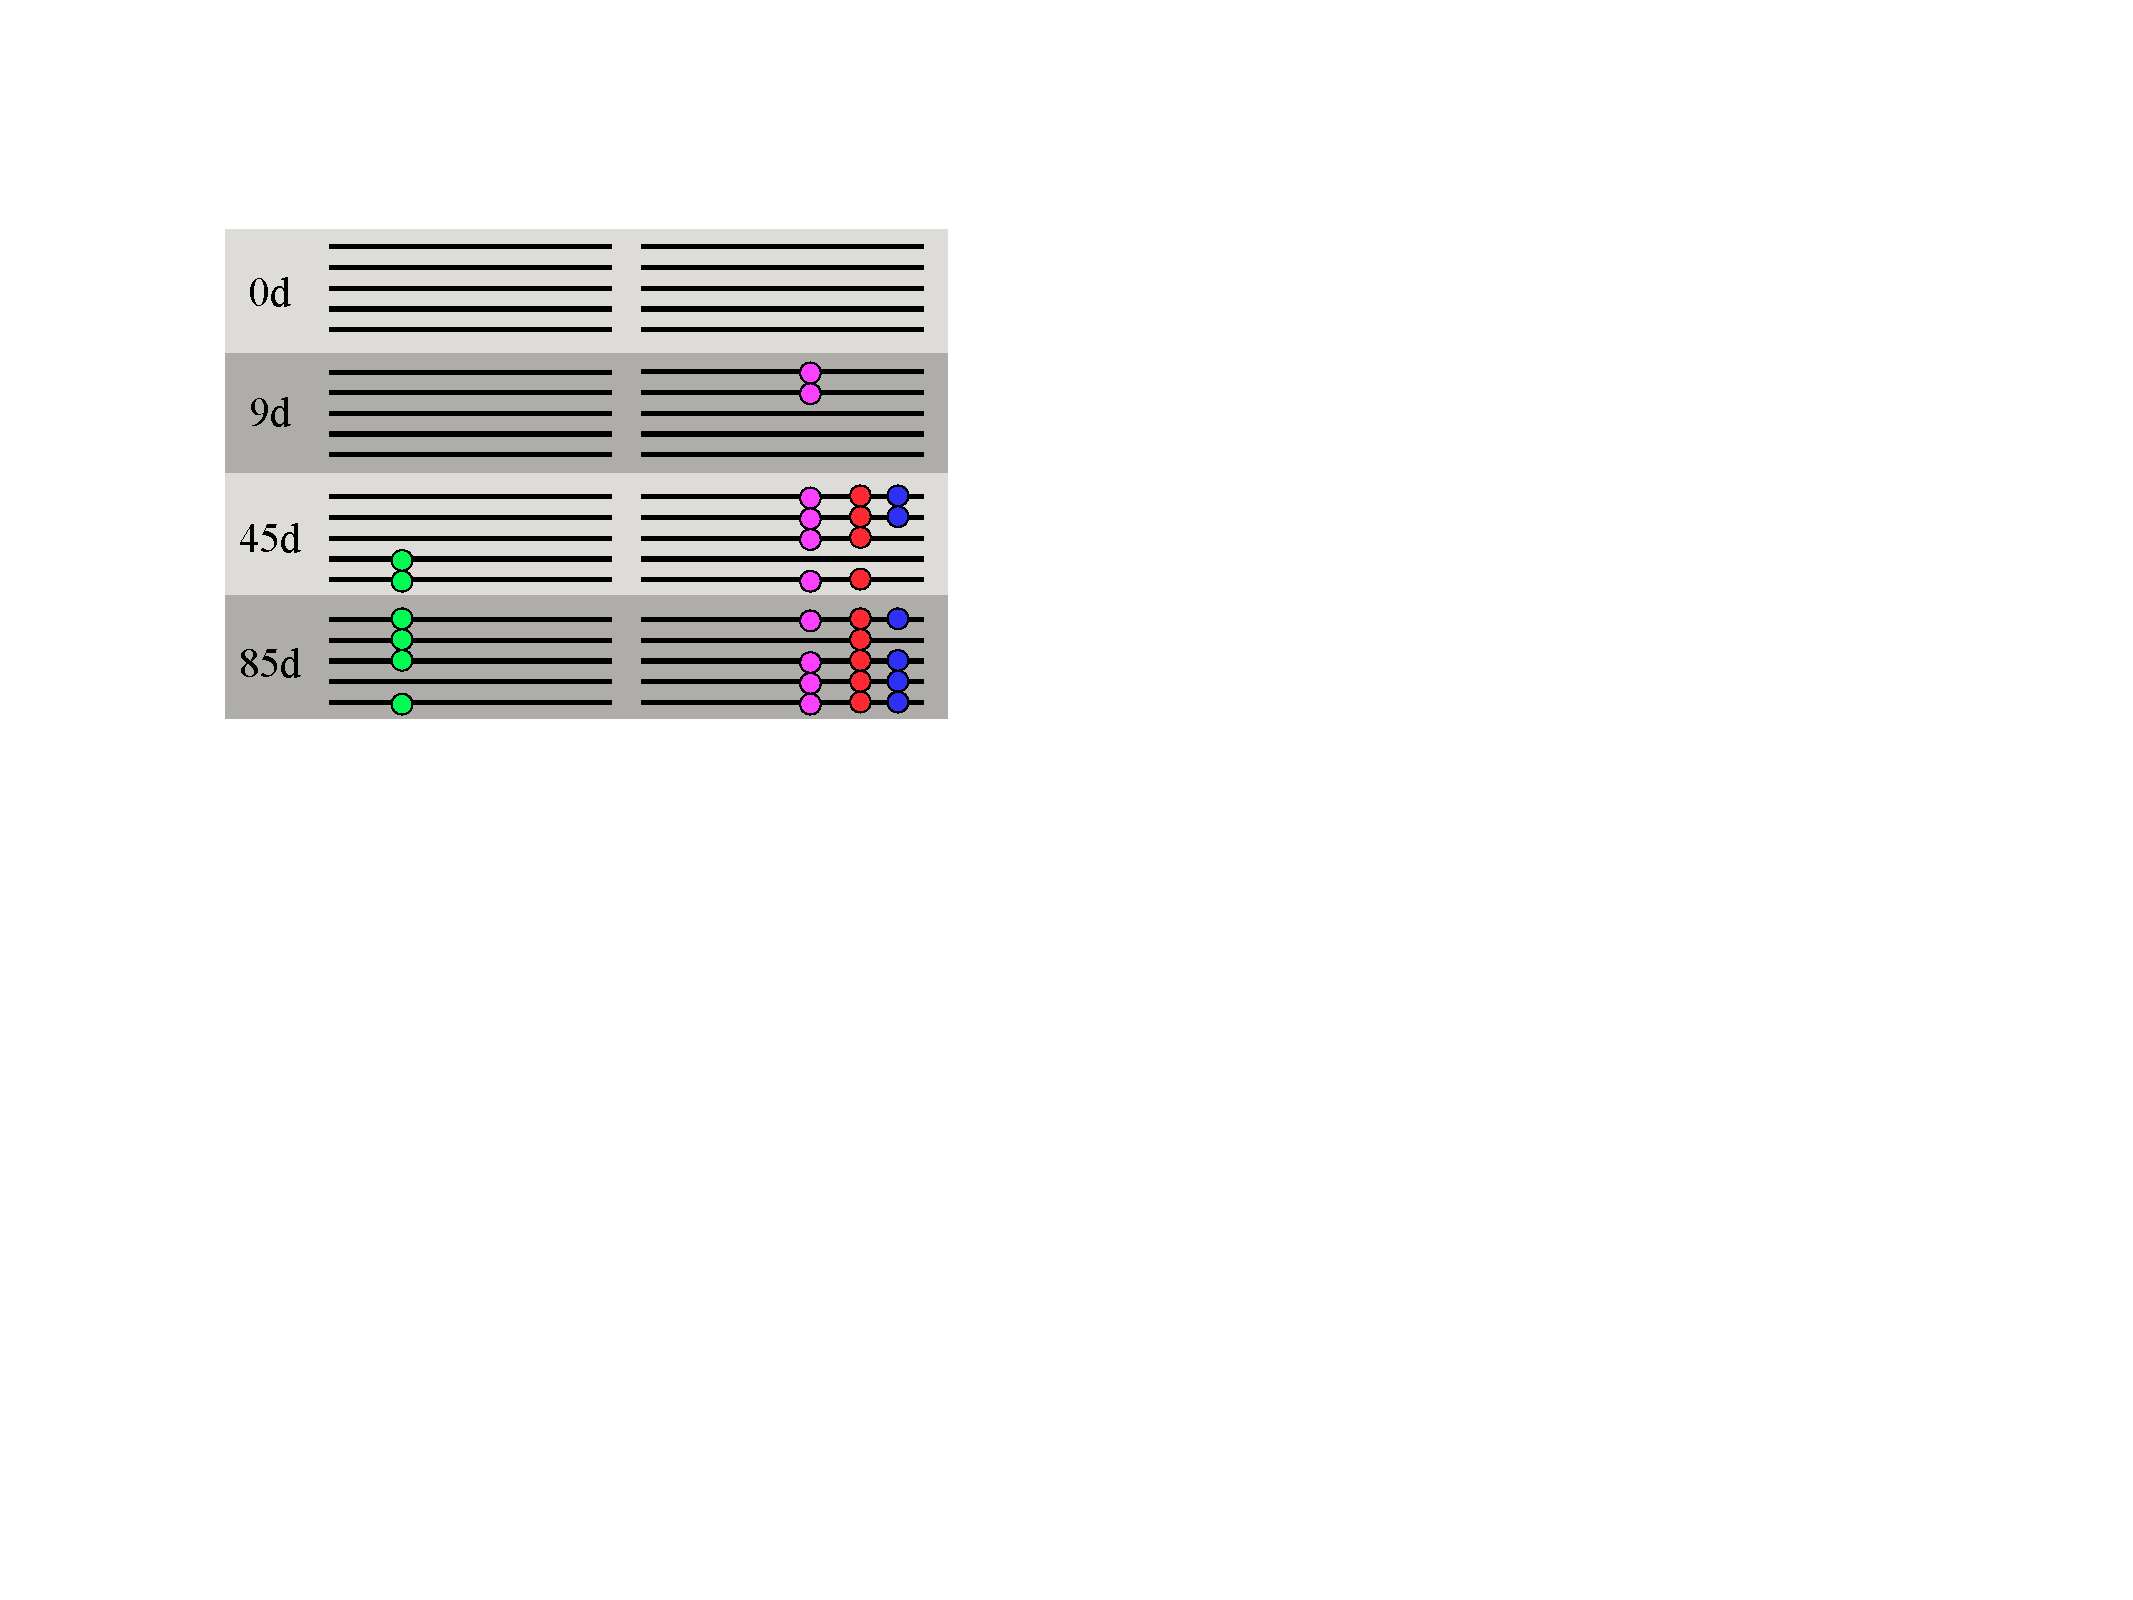
\includegraphics[width=0.48\columnwidth]{Figures/CH58_schematic}
  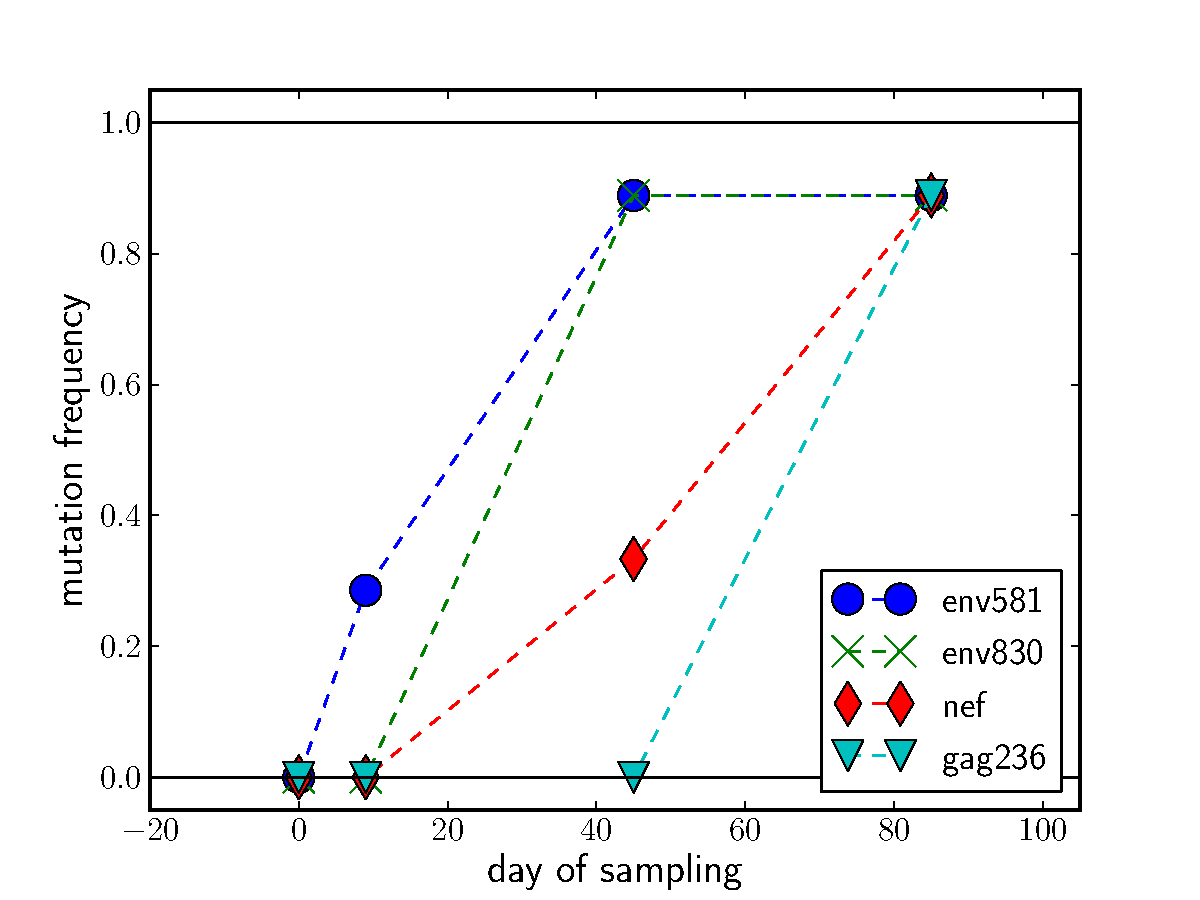
\includegraphics[width=0.48\columnwidth]{Figures/CH58_allele_freq_example}
  \caption[labelInTOC]{Escape from T-cell mediated immunity: The virus
  population in patient CH58 quickly acquires four substitutions. The left
  panel shows a sketch of genotypes at the first 4 escape mutations, observed
  at different times, see \citep{SalazarGonzalez:2009p35091,Goonetilleke:2009p42296} for the actual
  data. The right panel shows the frequenies of the mutations in samples of size 7 at day 9 and 9 at days 45
  and 85.}
  \label{fig:data_example}
\end{center}
\end{figure}

We will first define a model of the dynamics of escape mutations. This model
serves a two-fold purpose: it defines the parameter which we would like to
estimate from the data, and provides us with a computational tool to
investigate how the accuracy of the inference depends on sampling depth and
frequency, as well as how sensitively it depends on the values of parameters
such as mutation rates or population sizes. We reanalyze existing data of CTL
escape and find that accounting for mutli-locus effects in a finite population
results in higher estimates of the escape rates.

\section*{Model} In majority of HIV infections, a single founder virus is
transmitted resulting in an initially homogenous viral population
\citep{SalazarGonzalez:2009p35091}.
In the new host with a distinct set of MHC alleles and repertoire of T-cell
clones, a number of mutations $i\in \{1,\ldots,L\}$ are escape mutations that
reduce immune pressure. Assuming that the mutations have additive effects,
$\fcoeff_j$, the growth rate (birth rate minus death rate) is given by
\begin{equation}
F(\gt,t) = F_0(t) + \sum_i \fcoeff_i \locus_i
\end{equation}
where $\gt = \{\locus_1, \ldots, \locus_L\}$, $\locus_i \in \{0,1\}$ specifies
the genotype, and $F_0(t)$ accounts for a genotype independent modulation of
the growth rate. The latter could for example be due to variable numbers of
target cells. $F_0(t)$ controls the total population size, while the differences
between genotypes accounted for by $\sum_i \fcoeff_i \locus_i$ and result in
differential amplification of some genotypes over others. The
$\fcoeff_i$ are the quantities that we would like to estimate from the data. In
other words, the dynamics of relative genotype frequencies is governed by $\sum_i \fcoeff_i \locus_i$, 
while the dynamics of the total population size depends on $F_0(t)$
\citep{ganusov_mathematical_2013}. Within our model, mutations arise at rate
$\mu$ per base per generation. This rate can be epitope dependent. Our general
model of the HIV population includes recombination, which is assumed to happen
with rate $r$. In the event of recombination, all $L$ loci are reassorted. The
later is motivated by the reports of frequent template switching
\citep{Levy:2004p23309}, but an explicit genetic map could be implemented as
well.

We used FFPopSim \citep{zanini_ffpopsim:_2012} to simulate the model in
Python. The simulation stores the population $n(\gt,t)$ of each of the $2^L$
possible genotypes. In each generation, the expected changes of the $n(\gt,t)$
due to mutation, selection and recombination are calculated. The population of
the next generation is then sampled from these expected genotype frequencies
$\nu(\gt,t) = n(\gt,t)/N$.
The size of the population can be set at will each generation. This way, up to
15 epitopes can be simulated for 1000 generations within seconds to minutes. 

A typical realization of the population dynamics is shown in figure
\FIG{example}. As expected, the population is dominated by one genotype at every
time.
Furthermore, the mutations accumulate in order of their effect sizes and the new
dominant genotype arises from the previous by incorporation of the mutation with
the largest effect available. There are, however, many minority genotypes which
are rarely observed, see \FIG{example}B that shows the frequencies on a
logarithmic scale. We use these simulations to test the accuracy and robustness
of the inference procedure developed below.

%\usepackage{graphics} is needed for \includegraphics
\begin{figure}[htp]
\begin{center}
  \includegraphics[width=0.48\columnwidth]{Figures/dominant_gt}
  \includegraphics[width=0.48\columnwidth]{Figures/minor_gt}
  \caption[labelInTOC]{The population is dominated by one or two dominant
  genotypes and accumulates mutation sequentially. Nevertheless, the initial
  dynamics of each genotype is stochastic and there are many minor variants at
  any given time. This is best seen in the right panel where all 32 genotype
  frequencies are shown on a logarithmic scale. These rare variants are rarely
  sampled (genotype frequencies in samples of size ?? are indicated by the
  circles) and their noisy dynamics suggests that little information can be
  gained from them.}
  \label{fig:example}
\end{center}
\end{figure}

Of the many possible genotypes that are present at any moment, only a small
fraction is likely to be observed and relevant in the future. Simulations and
data suggest that the dominant genotypes accumulate mutations one by one -- this
is going to make the task of modeling the dynamics a lot easier. Instead of
modeling the dynamics of all possible genotypes ($2^L$), we will consider a
chain of genotypes each containing one additional mutation compared to its
predecessor. 



\section*{Inferring the escape rates}
Suppose we have obtained sequence samples of size $n_i$ at different time points
$t_i$ and each of these samples consists of different genotypes $\gt$ present in
$k(\gt,t_i)$ copies. If the actual frequencies of the those genotypes at
different times are $\nu(\gt,t_i)$, the probability of obtaining the sample at
$t_i$ is
\begin{equation}
P(\mathrm{sample}) = \frac{n_i!}{\prod_\gt
k(\gt,t_i)}\prod_{\gt}\nu(\gt,t_i)^{k(\gt,t_i)}
\end{equation}
If the underlying dynamics was deterministic, the frequencies $\nu(\gt,t)$
would be unique functions of the model parameters we want to estimate. In that
case we could use Bayes theorem, choose suitable priors, and determine the
posterior distribution of parameter values. However, the underlying model is stochastic and different
runs will provide different answers. Furthermore, most of the $2^L$ possible
genotypes remain unobserved. This leaves us with the choice of either
some type of approximate Bayesian computation that compares repeated simulations
of the model with appropriate summary statistics REF, or a reduced descriptions
of the observed genotypes only while the stochasticity is captured by nuissance
parameters.

In the case of selection for novel mutations, as considered here, the most
convenient quantity to capture the stochastic behavior is the time at which a
genotype that is destined to spread first appears. As soon as it reaches high
numbers, its trajectory is essentially deterministic and all the (unobserved) 
stochasticity can be captured by this seed time
\citep{Kepler:1995p26819,Desai:2007p954}.

\begin{figure}[htp]
\begin{center}
  \includegraphics[width=0.7\columnwidth]{Figures/model_vs_stochastic_sim}
  \caption[labelInTOC]{The deterministic model parameterized by seed times
  $\tau_i$ and selection coefficients $\fcoeff_i$ for the $L$ dominant genoytpes
  (solid lines) captures the dynamics of the stochastic model accurately
  (dashed lines). The trajectories (and seed times) vary from run to run.}
  \label{fig:model_vs_full}
\end{center}
\end{figure}

Assuming that only a sequence of dominant genotypes needs to be modelled, we
therefore face the problem of estimating $\fcoeff_j,\tau_j$ for $j=1,\ldots L$
from the data. This modified model parameterized by $\fcoeff_j,\tau_j$ tracks
only the dominant genotypes, denoted by $\nu_j(t)=\nu(\gt_j,t)$, which evolve
according to
\begin{equation}
\dot \nu_j(t) = F(\gt_j,t)\nu_j(t) +\mu [\nu_{j-1}(t) - \nu_{j}(t)]
\end{equation}
if $t>\tau_j$. Consersely, $\nu_j(t)=0$ for $t<\tau_j$. Genotypes are
seeded at $\nu_j(\tau_j)= (N\sigma)^{-1}$ at the seed time, where $\sigma$
accounts for the growth rate of the new genotype. If seed times are chosen
appropriately, this model provides a very accurate description of the frequency
dynamics of the dominant genotypes in the full stochastic model; see \FIG{model_vs_full}.

At face value, the deterministic model has two parameters per locus. The
seedtimes, however, are quite strongly constrained by basic facts of the
evolutionary dynamics. The a genotype $\gt_j$ carrying $j$ mutations arises with
rate $\mu N(t)\nu_{j-1}(t)$ from the genotype $\gt_j$ with $j-1$ mutations. This
means it unlikely that genotype $j$ arises early while $\nu_{j-1}(t)$ is still
very small, or very late when $\mu\int_0^tdt'\; N(t')
\nu_{j-1}(t')\gg 1$. Given the frequency trajectory of $\nu_{j-1}(t)$, the
seedtime $\tau_j$ should follow a distribution
\begin{equation}
\label{eq:seedtimes}
Q(\tau_j | \nu_{j-1}(t)) \approx \mu N(\tau_j)\nu_{j-1}(\tau_j) e^{-\mu
\int_0^{\tau_j}dt\; N(t)\nu_{j-1}(t)} \ .
\end{equation}
Note that a correction of the mutational influx for the establishment
probability is not necessary in this context as the same mutant is very rapidly
produced often ($N\mu\gg 1$).
Since the $\nu_j(t)$ are uniquely specified by $\tau_j,\fcoeff_j$, we can
write the posterior probability of the parameters as 
\begin{equation}
P(\{\fcoeff_j,\tau_j\})  \propto \prod_{i} P(\mathrm{sample}_i|\Theta)\prod_j
Q(\tau_j|\Theta)U(\fcoeff_j)
\end{equation}
where $\Theta = \{ \fcoeff_j,\tau_j\}_{j=1\ldots L}$ and $U(\fcoeff_j)$
reflects our prior on selection coefficients.


\section*{Obtaining maximum likelihood estimates} Traditionally, selection
coefficients have been estimated by fitting logistic curves to the
data\citep{Asquith:2006p28003,Ganusov:2011p43139}. The logistic curve has two
parameters, growth rate and initial frequency, which were estimated
independently for every sweeping locus.
However, estimating two parameters from infrequently sampled data is often
impossible and the resulting estimates are rather noisy. In essence, this
strategy works only when a genotype is sampled at least twice at intermediate
frequencies. On top of that, assuming that different loci are independent is
often inadequate, as can be seen by the changing slope of the log-frequency of
many genotypes in simulations, see \FIG{example}.

While our model also has two parameters per locus, the seed times are quite
drastically constrained by the seedtime prior, which effectively reduces the
degrees of freedom.
Nevertheless, finding the set of parameters that maximizes the posterior can be
rather difficult due to multiple maxima and ridges in the high dimensional
search space and uncertainty remains.

To ensure a reliable discovery at the global optimum, one can employ the
sequential nature of the dynamics and use the fact that earlier sweeps
strongly affect the timing of the later ones, but not vice versa. Thus adding
genotypes with increasing number of mutations one at a time 
results in a pretty good initial guess on top of which a global true multi-locus search can be
performed. 

We have implemented such a search in Python, while the computationally expensive
calculation of the posterior probability is done in C. The code infers
parameters as follows:
\begin{itemize}
  \item fit the first substitution assuming $\tau_1=0$ by a
  simple one dimensional minimization. 
  \item Add additional loci successively by mapping the entire two-dimensional
  posterior distribution $P(\fcoeff_j,\tau_j)$ at fixed $\{\fcoeff_k,\tau_k\}$
  for $k<j$. This step is illustrated in \FIG{sequential_fitting}A.
  \item Refine estimates through local optimization via gradient descent, Monte
  Carlo methods, or local exhaustive search. The resulting parameters and
  trajectories are shown for one example in \FIG{sequential_fitting}B.
  \item generate posterior distributions by Markov chain Monte Carlo. 
\end{itemize}
This procedure is fast and runs one the order of a minute including the
generation of (local) posterior distributions by MCMC.

In an inference problem of this sort, one has to weigh the data against
prior belief. We employ a Laplace prior favoring small selection coefficients.
The prior regularizes the search of the minimum and results in conservative
estimates of selection.



%\usepackage{graphics} is needed for \includegraphics
\begin{figure}[htp]
\begin{center}
  \includegraphics[width=0.9\columnwidth]{Figures/sequential_LH}
  \includegraphics[width=0.9\columnwidth]{Figures/sequential_traj_refined}
  \caption[labelInTOC]{Adding loci one by one is a feasible and reliable
  fitting strategy. Assuming we know the population was homogeneous at $t=0$,
  there is only one free parameter for the first locus, which is easily
  determined.  For all subsequent loci, we need to determine the seed time
  $\tau_i$ and the selection coefficient $\fcoeff_i$. The negative log posterior
  probability of these parameters is shown for each of the loci. The surface
  typically exhibits a single minimum, often at the bottom of a narrow valley. 
  The second panel shows the trajectories that correspond to the estimated
  parameters (solid lines) in comparison to the actual genotype frequencies
  (dashed lines) and the samples (circles, 20 sequences at each time point). }
  \label{fig:sequential_fitting}
\end{center}
\end{figure}

\section*{Comparison to simulated data}
To evaluate the accuracy and reliability of our inference scheme, we simulated
our model under a variety of conditions and compared the inferred parameters to
their actual values. In essence, there are two sources of error:
Limited sample size and sampling frequency will incur errors due
inaccurate estimates of the actual genotype frequencies from the
sample. The second source of uncertainty is an inappropriate choice
of model or model parameters. Such inappropriate model choices might include
wrong estimates of the population size, mutation rates, presence/absence
of recombination, or time variable CTL activity.

We generate data assuming selection coefficients $f_j = 0.4, 0.3, 0.2, 0.08,
0.04$ and sample the population on days $t_i=0, 15,30,60,120,250,400$. An
example of such samples is shown in \FIG{example}. Note that each genotype
is typically only sampled at a single data point and that it easily happens that
a genotype is hardly seen at all. We therefore expect all inferences to be quite
noisy.

\subsection*{Sample size and sampling frequency dependence} 
With more frequent and deeper sampling, inferring the model parameters is
expected to become simple. Indeed, as soon as each genotype is sampled more than
once at intermediate frequency, one can estimate its growth advantage simply
from its rate of increase. This is the rational behind previous studies such as
\citep{Asquith:2006p28003,Ganusov:2011p43139}. In most data sets, however, this
condition is not met. By constraining the seed-time based on the evolutionary
trajectory of the previous sweep, our method is able to produce a more accurate
reconstruction of parameters with less data. 


\FIG{sample} shows the estimates obtained as a function of the sampling
frequency and sample size. Increasing the sample size improves the estimates
only moderately, while increasing the sampling frequency leads to substantial
improvements.

%\usepackage{graphics} is needed for \includegraphics
\begin{figure}[htp]
\begin{center}
  \includegraphics[width=0.48\columnwidth,type=pdf,ext=.pdf,read=.pdf]{Figures/sample_size_prior_F_10.0_S_1.0_multi_locus_normed}
  \includegraphics[width=0.48\columnwidth,type=pdf,ext=.pdf,read=.pdf]{Figures/sampling_interval_prior_F_10.0_S_1.0_multi_locus_normed}
  \includegraphics[width=0.48\columnwidth,type=pdf,ext=.pdf,read=.pdf]{Figures/sample_size_prior_F_10.0_S_1.0_samplesize_100.0_histogram}
  \includegraphics[width=0.48\columnwidth,type=pdf,ext=.pdf,read=.pdf]{Figures/sampling_interval_prior_F_10.0_S_1.0_samplesize_10.0_histogram}
  \caption[labelInTOC]{The dependence of the accuracy of inference on sample
  sizes and sampling intervals. Sample size only moderately affects the
  accuracy, while to sparse sample (every 40 days in this example) leads to
  serious loss of accuracy. The lower two panels show the distributions of
  estimates for all coefficients at the highest sample size (left, $n=100$) and
  the most frequent sampling (right, $\delta t = 10$days). Sample size is
  $n=20$ when sample intervals are varied, and sampling times are as
  illustrated in \FIG{example} when sample size is varied. The plots show the
  mean, while error bars are interquartile distances.}
  \label{fig:sample}
\end{center}
\end{figure}


\subsection*{Model deviations}
The population size and the mutation rate explicitly enter our model through the
seedtime prior. A larger product $N\mu$ favors earlier seeding of subsequent
genotypes, which in turn results in smaller selection coefficients. We varied
$N$ and $\mu$ and observed the expected effect on the estimates, as shown in
\FIG{modeldeviation}. However, the dependence on $N\mu$ is rather weak and
varying $N$ or $\mu$ over several orders of magnitude only changes the estimated
selection coefficients by $\pm 50\%$.
The underlying reason is that most time scales involved depend on $\log N$
rather than $N$ due to the exponential amplification by selection. The
dependence on $\mu$ is somewhat stronger than that on $N$ because the mutation
rate not only affects the time of seeding, but also the initial rise in
frequency of rare mutation due to recurrent mutations.

Another factor that affects seedtimes is recombination. HIV recombines 
via template switching following coinfection of one target cell by several virus
particles \citep{Levy:2004p23309}. In chronic infection, coinfection happens
with a frequency of about 1\% \citep{Neher:2010p32691,Batorsky:2011p40107}. Recombination is
not modeled in our seedtime prior, but can nevertheless produce novel genotypes by
combining mutations that arose in different cells. As a result, if recombination
is present, seeding tends to happen earlier then expected on the basis of our
prior, which results in overestimates of the selection coefficients. This is
shown in \FIG{modeldeviation}. Recombination starts to have substantial effects
once coinfection exceeds a few percent. Recombination primarily affects the
incorporation of more weakly selected mutations and can be ignored for very
strongly selected CTL escape mutations. 

%\usepackage{graphics} is needed for \includegraphics
\begin{figure*}[htp]
\begin{center}
  \includegraphics[width=0.65\columnwidth]{Figures/popsize_prior_F_10_S_1_samplesize_20_multi_locus_normed}
  \includegraphics[width=0.65\columnwidth]{Figures/mutrate_prior_F_10_S_1_samplesize_20_multi_locus_normed}
  \includegraphics[width=0.65\columnwidth]{Figures/recrate_prior_F_10_S_1_samplesize_20_multi_locus_normed}
  \caption[labelInTOC]{The effect of assuming the wrong population parameters
  on the escape rate estimates. A) Assuming to large population sizes
  results in estimates that are too low. B) Similarly, if the mutation rate is
  assumed too large, the estimated seeding of multiple mutants occurs too late,
  and results in low estimates.
  C) If the actual population recombines, seeding occurs earlier
  than estimated, and estimates of selection coefficients go up. This effect is
  most pronounced for the weakly selected loci. }
  \label{fig:modeldeviation}
\end{center}
\end{figure*}


\subsection*{Unobserved intermediates and compensatory mutations}
The time intervals between successive samples are sometimes to large to observe
the accumulation of single mutations, but the dominant genotype at the later
time point differs by more than one mutation from the previous. This can arise
for two reasons: One or several unobserved genotype which were transiently at
high frequency but got outcompeted by later genotypes. Alternatively, one escape
might have required more than one mutation to begin with, for example because
single mutants are not viable and a compensatory mutation is needed
\citep{read_stochastic_2012}. Both scenarios can be accounted for in our scheme. 

Unobserved, but individually beneficial, intermediate genotypes can be included
by assuming they all have the same coefficient and got seeded one from the
other. Obviously, there is no information to estimate more than an average
selection coefficient for all of them. For a given set of sampled frequencies,
the estimated selection coefficients increase, as more and more intermediates
are assumed.

Compensatory mutation and ``multiple-hit'' escapes can be accounted for by
replacing the single site mutation rate by the effective rate to the viable
escape mutant in \EQ{seedtime}. In the simplest case where all intermediate
states are lethal and mutations are independent, this rate is simply the probability $\mu^k$,
where $k$ is the number of mutations needed. In other cases, the rates to
multiple hits can be calculate using branching process approximations
\citep{Weissman:2009p23398,Neher:2011p42539}.



\section*{Immune escape in HIV -- reanalysis of CTL escapes in subject CH58}
In many ways, the data collected and analyzed in
\citep{SalazarGonzalez:2009p35091,Ganusov:2011p43139} is sparser and less
densely sampled than most of the examples analyzed above and any estimates are
necessarily rather inaccurate. Furthermore, we don't know when exactly infection
happened or CTL selection started. Assuming selection started 20 generations
before the first sample, a mutation rate of $\mu=10^{-5}$ and a population size
of $N=10^6, \;10^8, 10^{10}$, we obtain posterior distributions for the
selection coefficients, all shown in \FIG{patients}. The population size is
expected to be around $N=10^8$ infected cells per day
\citep{Perelson:1996p23158}, while the mutation rate is on the order of
$10^{-5}$ \citep{Mansky:1995p38971}. Recombination in HIV occurs, but not
modelled here since its rate is low \citep{Neher:2010p32691,Batorsky:2011p40107}
and it is expected to be less revelevant for the strong escapes than recurrent
mutations. Nevertheless, the neglect of recombination leads to a tendency to
overestimate the rate of escape.

From \FIG{patients}, we see that larger the population
sizes result in smaller estimates of the escape rates,  as expected from
\FIG{modeldeviation}.
The population sizes $10^8$ and $10^{10}$ are large enough to make instantaneous
double mutants possible, which reduces the seedtimes dramatically.

%\usepackage{graphics} is needed for \includegraphics
\begin{figure}[htp]
\begin{center}
  \includegraphics[width=0.95\columnwidth]{Figures/CH58_F_10_S_1_tau_20_posterior}
  \caption[labelInTOC]{The posterior distribution of the escape rates for
  for different population sizes. For comparatively small populations, the
  distribution are very broad since seeding of mutliple mutants remains very
  stochastic and happens later, such that high selection coefficients are
  required to match the data. It is assumed that CTL selection starts 20 days
  prior to the first sample and the fitness prior as weight 10.}
  \label{fig:patients}
\end{center}
\end{figure}


While the posterior distributions are quite broad, they nevertheless suggest
that escape rates can be substantially higher than previously estimated. Furthermore, they
no longer decay as strongly with later appearance. The underlying reason for
this is that selection on the a late escape is really only active after the
successful multiple mutant has been produced. In previous single locus
estimates, selection was allowed to act on the mutant frequency from the very
beginning, resulting in a reduced estimate of the escape rate. 

\section*{Discussion}
We have suggested a way to infer coefficients from sparsely sampled time series
of the evolutionary dynamics of asexual or rarely sexual populations such as
HIV. We exploit the sequential nature at which mutations are accumulated, which
allows us to constraint the times at which new mutations arose. These
constraints regularize the inference to a large extend, but additional stability
and parsimony is gained by prioritizing small selection coefficients.

Reanalysis of CTL escape data from HIV using our method suggests that CTL
escapes are sustantially more rapid than previously thought. Furthermore, the
relevant ``effective'' population size needs to be much larger than most
estimates in the literature. The population is relevant in finding the required
mutliple mutants quickly and simulations suggest that population sizes in excess of
$10^6$ are required. This population size has very little to do with genetic
diversity in the population, which is often use to define the ``effective''
population size. 

Similar bursts of successive mutations are believed occur during the development
of cancer. If the rate at which these mutations occur is small, the individual substitutions
are well separated in time, i.e., the time it takes one mutation to spread
through the population is small compared to the waiting time for the next
mutation. In many populations of interest, in particular HIV with its large
mutation rate, mutations compete against each other and double or triple
mutant genomes are formed before the previous mutation has
swept to high frequency \citep{Desai:2007p954,Beerenwinkel:2007p23640}. This
competition between genotypes is also important in populations that only rarely
reproduce sexually as for example many viral populations
\citep{Neher:2009p22302,Neher:2011p42539}.



\bibliography{bib}
\end{document}